\section{Laser}
\subsection{Funktionsweise eines Lasers}

Ein Laser ist ein Gerät, welches nach dem gleichnamigen Prozess, der den Lichtstrahl des Lasers erzeugt, benannt ist. Das Herzstück des 
Lasers ist der optische Resonator (siehe Abb. \ref{bild:LaserAufbau}). Dieser ist im Allgemeinen ein Material, was die Energie des elektromagnetischen Feldes speichern kann. Dies 
geschieht meistens als stehende Welle, also wenn die Länge $L$ des Resonators 

\begin{equation}
    L = N\cdot\frac{\lambda}{2}
\end{equation}

ein Vielfaches der halben Wellenlänge ist. Die Photonen wandern also in dieser stehenden Welle durch den Resonator. Nun werden sie an den Enden
des Resonators von, hier konfokalen, Spiegeln reflektiert. \\
Damit die Photonen im Resonator mehr werden, benötigt man die stimulierte – oft sagt man auch induzierte – Emission. Diese führt dazu, dass ein Photon 
bei einem Durchlauf ein weiteres auslösen kann. Die für das Vermehren der Photonen benötigte Energie wird von der Pumpe geliefert. Diese kann optisch 
oder elektrisch funktionieren.\\

\begin{figure}[ht]
    \centering
    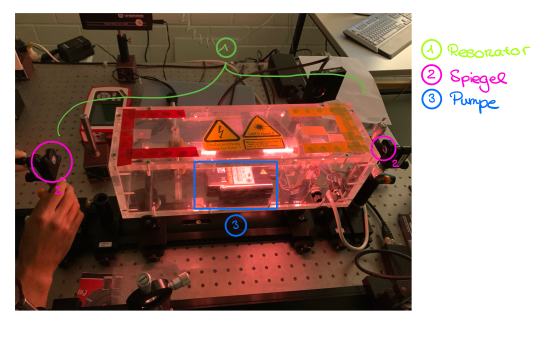
\includegraphics[width = 14cm]{Bilder/Auswertung/LaserAufbau.png}
    \caption{Elemente eines Lasers an unserem HeNe-Laser erklärt}
    \label{bild:LaserAufbau}
\end{figure}

Die Energie im elektromagnetischen Feld reduziert sich durch die Absorption im Resonator und durch das Austreten von Photonen an einem Spiegel.
Der Spiegel ist leicht durchlässig gebaut. Die Besonderheit des austretenden Lichtes ist, dass es in Phase, vergleichsweise konstant in seiner Leistung, spektral 
schmalbandig und oft polarisiert ist. Dies alles macht einen Laser zu einer guten Lichtquelle für die Anwendung im Labor. 

\clearpage
\subsection{Drei-/Vierniveaulaser}

Um den Laser zu realisieren muss das obere der am Strahlungsprozess beteiligten Niveaus immer gut gefüllt sein. Man spricht
hierbei von einer Inversionslage. Für die Erzeugung einer solchen muss man weitere Hilfszustände
einführen. Bei einem Vierniveaulaser (siehe Abb. \ref{vrei}) hat man zwei weitere Hilfsniveaus, eines unter dem Grundzustand und eines über dem Grundzustand. 
Damit kann man einen Dauerstrichlaser aufrecht erhalten, da die Inversionslage aufrecht erhalten werden kann. \\
Ein Dreiniveaulaser (siehe Abb. \ref{drei}) hat nur ein weiters Hilfsniveau, nämlich das unter dem Grundzustand. Bei beiden Lasern pumpt man auf
das höchste Energieniveau. 

\begin{figure}[ht]
    \centering
    \subfloat[Dreiniveaulaser]{\label{drei}%
    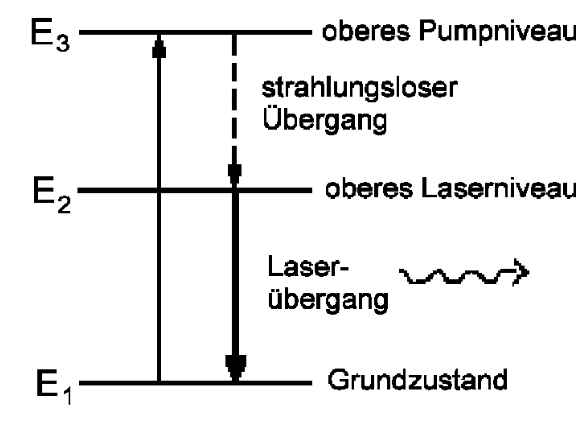
\includegraphics[width=0.35\textwidth]
    {Bilder/Auswertung/3NiveauLaser.png}}\quad
    \subfloat[Vierniveaulaser]{\label{vrei}%
    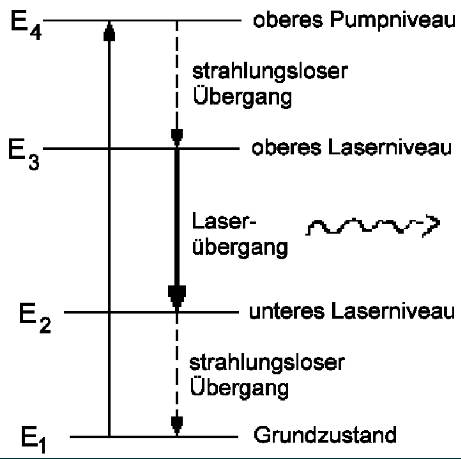
\includegraphics[width=0.25\textwidth]
    {Bilder/Auswertung/4NiveauLaser.png}}
      \caption{Drei- und Vierniveaulaser schematisch dargestellt \protect \footnotemark}
      \label{bild:LaserNiveaus}
\end{figure}

\footnotetext{Quelle: \url{http://www.pci.tu-bs.de/aggericke/PC4/Kap_III/Laser.htm} eingesehen 09.10.2021}

\subsection{Spontane und stimulierte Emission}

Es existieren zwei Arten von Emission. Das zugrundeliegende Prinzip erklären wir an der spontanen Emission. Ein Photon wird emittiert, wenn ein Elektron 
von einem höheren in ein niedrigeres Energieniveau übergeht. Wie lange der angeregte, höherenergetische Zustand bestehen bleibt, lässt sich nicht vorhersagen. Man kann aber im Allgemeinen 
eine Energie-Zeit-Unschärfe abschätzen, wie Heisenberg es getan hat, und ansetzten, dass 

\begin{equation*}
    \Delta E \cdot \Delta t \sim  \hbar
\end{equation*}

die Zeit invers proportional zur Energie des angeregten Zustandes ist.\\
Die spontane Emission ist unabhängig von außeren Faktoren, wenn es darum geht, wann das Photon emittiert wird; es muss
nur ein angeregtes Atom vorhanden sein. Die spontane Emission ist wichtig um den Laser zu starten. Von ihr stammt das erste Photon, was dann 
durch stimulierte Emission vervielfacht wird.\\
Bei der stimulierten Emission läuft der selbe Prozess wie oben beschrieben ab, jedoch wird der Übergang des Elektrons in ein niedrigeres Energieniveau
durch ein vorbeifliegendes Photon stimuliert. Das bei diesem Übergang freiwerdende Photon ist in Phase mit dem ersten Photon. Man hat also aus einem Photon
zwei Photonen gemacht, welche in Phase sind, wie in Abbildung \ref{bild:Emission} zu sehen.

\begin{figure} [ht] 
    \centering
    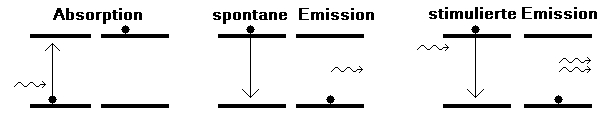
\includegraphics[width = 13cm]{Bilder/Auswertung/Emission.jpg}
    \caption{Prozess der Absorption, spontanen Emission und stimulierten Emission\protect \footnotemark}
    \label{bild:Emission}
\end{figure}

\footnotetext{Quelle: \url{https://illumina-chemie.de/upload/30_66180837749063cd2437ad.jpg} eingesehen am 09.10.2021}

\subsection{Lasermoden}
\label{subs:moden}

Das Licht bildet in dem Resonator eine stehende Welle. Wie bei jeder stehenden Welle gibt es 
auch beim Laser Moden, hier transverale und axiale.

\subsubsection{Transverale Moden}

Die Moden, welche einfach zu beobachten sind, sind die transversalen Moden. Diese sind durch eine Veränderung des
Strahlenprofils im Ausgang beobachtbar. Da die Symmetrie des Resonators durch die 
Ausrichtung der Brewsterfenster verschwindet, sieht man in x- und y-Richtung aufgespaltene Moden. Diese werden anhand der Notation $TEM_{nm}$ benannt.
Dabei ist $n$ die Anzahl der Nullstellen in x-Richtung und $m$ die Anzahl der Nullstellen in y-Richtung. Man kann die Moden auch
erzwingen, indem man wie wir in dem Versuchsteil \ref{section:transvM} eine Drahtblende einsetzten.


\subsubsection{Axiale Moden}

Axiale Moden kommen aus der Wechselwirkung des Strahles mit sich selbst.
Dabei existieren im Resonator nur stehende Wellen, aber diese können unterschiedlich viele Knotenpunkte haben, bis 
die Welle insgesamt wieder an ihrem Ursprungspunkt, beispielsweise einem Knotenpunkt an einem Spiegel, in gleicher Phase ankommt. Da wir es mit einem konfokalen Resonator (siehe Abb.\ref{bild:Konfokal}) zu tun haben,
ergibt sich also die Länge 
\begin{equation}
    L \overset{!}{=} k \cdot \frac{\lambda}{4n},
\end{equation}
wobei $k$ eine frei wählbare ganze Zahl ist und $n$ der Brechungsindex des Resonatormediums.
Betrachtet man nun zwei benachtbarte $k$ so stellt man fest das der Frequenzabstand 

\begin{equation}
    \Delta \nu = \frac{c}{4L\cdot n}
    \label{eq:FSR}
\end{equation}

ist, welcher für alle benachtbarten $k$ gleich ist.\\
Dieser Frequenz-/Modenabstand ist mit dem bloßen Auge nicht zu erkennen. Daher verwendet man ein Fabry-Pérot-Interferometer, was in Abschnitt \ref{section:Fabry} genauer behandelt wird.

\begin{figure}[ht]
    \centering
    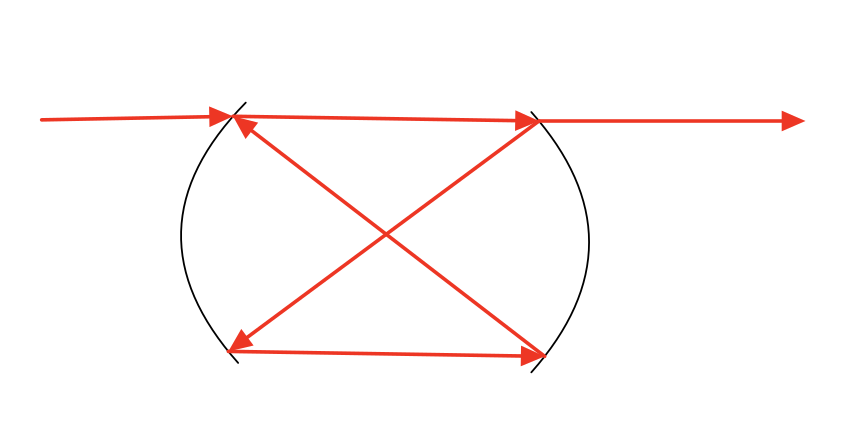
\includegraphics[width = 8cm]{Bilder/Auswertung/KonfokalSpiegel.png}
    \caption{Konfokale Spiegel und der damit Verbundene Strahlengang. Man sieht schön, dass der Stahl viermal die Länge $L$ überwinden muss, um am Ausgangspunkt wieder anzukommen}
    \label{bild:Konfokal}
\end{figure}